\section{\label{III-A-1}La représentation conceptuelle : modéliser pour maîtriser la complexité}

\subsection{Les enjeux de la modélisation conceptuelle}

Comme démontré plus haut dans la rapide présentation des vocabulaires utilisés au \mae, la masse de données à traiter est considérable\footnote{Voir le tableau \refinterne{tab:thesaurus_synthese}}. Ces données se présentent toutes sous la forme de tableurs excel exportés des différents logiciels de gestion du vocabulaire, et analyser leur structure et en déduire une méthodologie à suivre pour les optimiser est un réel défi pour le cerveau humain
Avant tout projet d'unification, visualiser les données pour pouvoir mieux les appréhender s’impose donc comme un nécessité : en effet, en les mettant à plat les et en permettant à l'utilisateur de les visualiser et de les embrasser dans leur ensemble, il est possible de rendre plus manifeste la structure des connaissances, de faire apparaître ce qui se cache dans l’enchevêtrement des termes, des usages et des hiérarchies.
Dans son article \citetitle{arruabarrenaDatavisualisationPrincipesEnjeux2015}, \citeauthor{arruabarrenaDatavisualisationPrincipesEnjeux2015} explique les enjeux et la nature d'une visualisation de données (\textit{datavisualisation} en anglais). La \textit{datavisualisation}, écrit-elle, \enquote{n’est rien d’autre qu’un processus de dévoilement qui vise à rendre visible une partie du monde au travers d’un dispositif sociotechnique}. En s'appuyant sur les idées de chercheurs comme le psychologue Michel Denis\footcite{denisImageCognition1989} ou l'anthropologue Jack Goody\footcite{goodyDomesticationSavageMind1977}, elle rappelle que cette manière de \enquote{représenter le monde dans sa complexité\footcite{arruabarrenaDatavisualisationPrincipesEnjeux2015}} s'appuie sur notre système cognitif pour \enquote{rompre avec la lecture linéaire du texte [en] l’illustrant, le démontrant, voire le remplaçant totalement\footcite{arruabarrenaDatavisualisationPrincipesEnjeux2015}}. C'est, rappelle-t-elle, \enquote{un \enquote{dispositif spatial de triage de l’information\footcite{goodyDomesticationSavageMind1977}} qui par des modalités graphiques d’organisation des données (listes, tableaux, inventaires, registres, etc.) facilite sa représentation, sa mémorisation, et donc sa réorganisation\footcite{arruabarrenaDatavisualisationPrincipesEnjeux2015}.}

Lorsque fut lancé au \mae le projet de rationalisation des \gls{thesaurus} et vocabulaires contrôlés du musée, dont notre stage a été l'un des premiers jalons, la première étape, après avoir pris connaissance des données -- mais également pour mieux les connaître -- a immédiatement consisté en la réalisation de graphes d’arborescence pour chaque lexique, à l’aide du logiciel \textit{Gephi}, de représentations générales de la structure de ces vocabulaires en UML ou sous forme de \textit{mindmaps} afin de visualiser et comparer leurs structures générales. C'est cette visualisation qui a notamment permis de révéler l’existence de termes orphelins, de clusters thématiques isolés, ou d’incohérences de rattachement qui rendaient difficile l'accès à certains termes. [TODO : voir figure à ajouter à la fin du mémoire.] Le travail de modélisation a ainsi permis de remettre au jour ces impasses sémantiques et d’envisager une restructuration cohérente.

Gérer l'information, en musée ou ailleurs, revient à une forme de gestion des données : comme le démontrent les articles de projets en institution patrimoniales, toute manipulation de données à grande échelle sous-entend cette étape. Les choix de modélisations, les outils et les manières de faire sont cependant extrêmement diverses et peuvent varier d'un projet à l'autre : si, au musée, le choix a été fait de commencer par ces visualisations manuelles afin de déterminer une base de travail pour les projets ultérieurs, la plupart des projets en institutions patrimoniales se sont tournés vers des standards universels comme le \ac{rdf}, qui permettent notamment de générer des graphes aisément manipulables et explorables après conversion\footcite{bermesCasLierDonnees2013a,bermesConvergenceInteroperabiliteLapport2011,filabesLindexationRAMEAUAssistee2025,reichThesaurusAuGraphe2022}[TODO : trouver un autre exemple avec des modélisations classiques].


La modélisation en effet n'est pas seulement un outil technique, mais un véritable instrument de gouvernance intellectuelle. Clarifier les hiérarchies, identifier les termes orphelins ou doublons, faciliter le dialogue entre métiers : la modélisation conceptuelle prépare le terrain à une transmission des savoirs, et à la constitution d’un langage commun qui transcende la division des métiers et des utilisateurs.


\subsection{Outils et méthodes de modélisation}


La typologie des outils disponibles est désormais bien établie. Les diagrammes UML qui sont aujourd'hui devenus des standards dans la formalisation des systèmes d'information, s'imposent par leur rigueur et leur capacité à modéliser des relations complexes. Dans notre cas, ils permettent notamment de distinguer nettement les différents types de vocabulaires : thésaurus de mots-clés, listes d'autorités pour les événements, les personnes, ou encore les lieux. Leur formalisme offre une grande cohérence et une intéropérabilité précieuse : la norme ISO 25964 est ainsi accompagnée d'une modélisaiton en UML du thésaurus idéal et aux normes. En mettant en miroir cette modélisation avec l'une tirée des données du musée, il est ainsi possible de repérer les divergences d'avoec les normes, de voir ce qui pourraiet être ajouté à l'existant, en bref, de montrer plus concrètement ce qui pourrait être réalisé avec l'existant grâce à cette norme\footnote{Voir en l'annexe \refinterne{Ax-F}}.



Pour autant, l'expérience du terrain montre que ces modèles, s'ils sont puissants, ne sont pas toujours adaptés à la diversité des publics et des usages. Les schémas UML nécessitent en effet une compréhension des codes utilisés : jugés « obscurs » ou trop abstraits par les agents de conservation ou les usagers non spécialisés, ils se sont révélés de moindre utilité que d'autres formats. 

\begin{figure}[htbp]
	\centering
	\begin{subfigure}{0.45\textwidth}
		\centering
		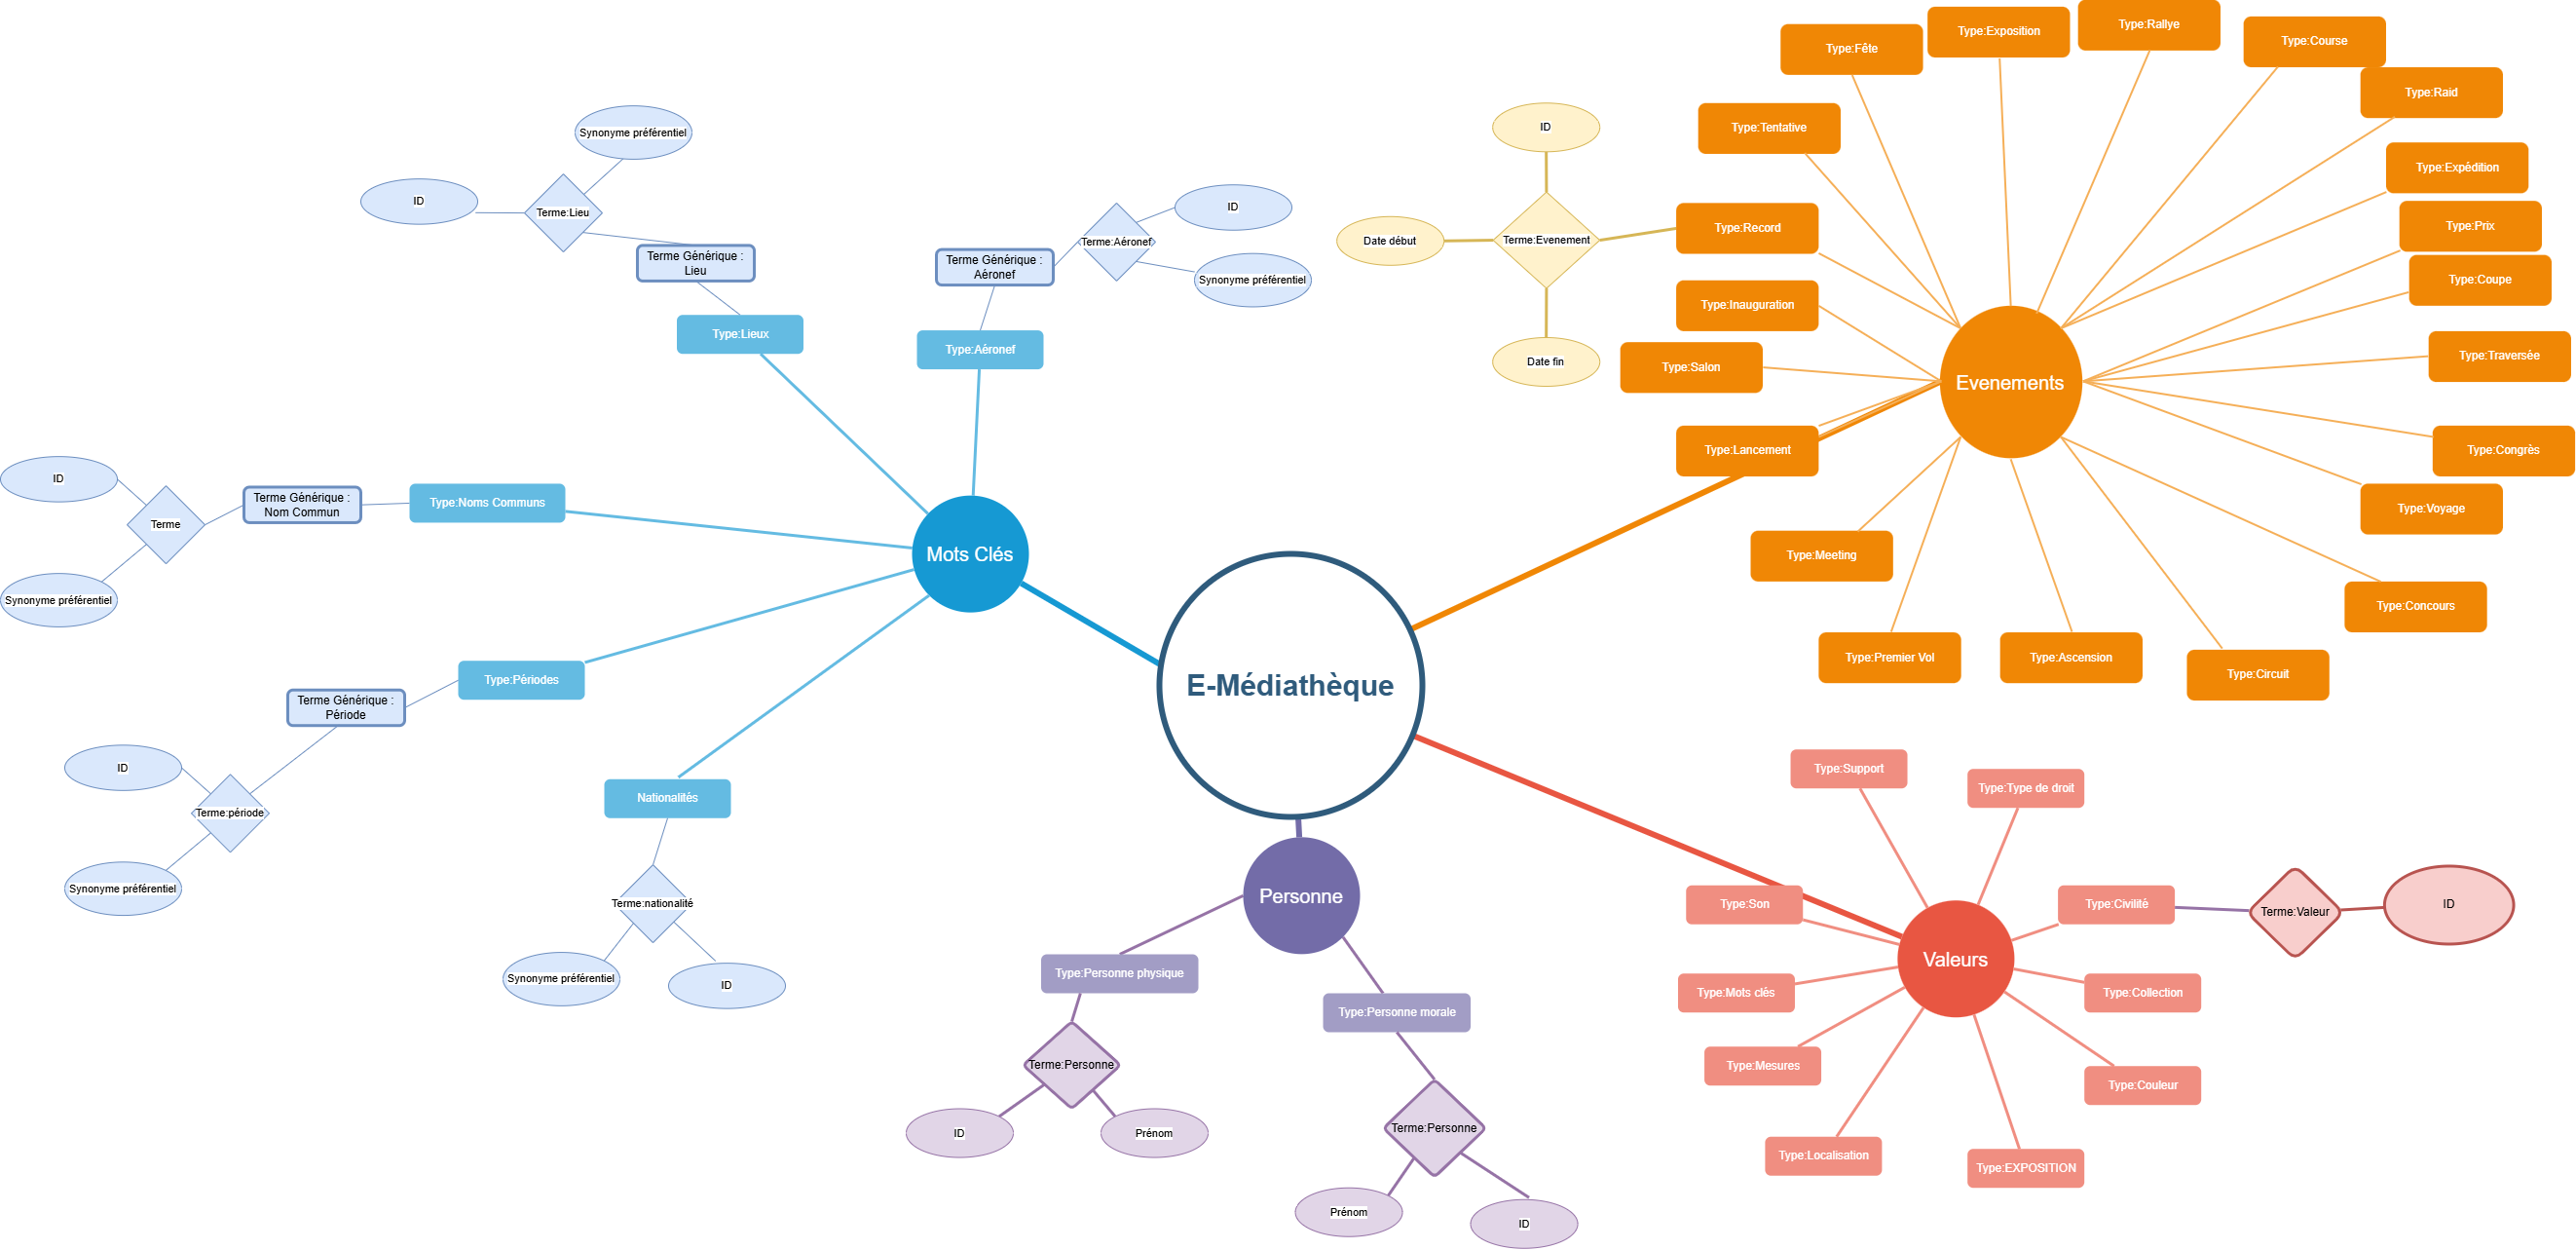
\includegraphics[width=\linewidth]{img/MODEL_emediatheque_mindmap}
		\caption{Modélisation en \textit{mindmap} réalisée avec \textit{draw.io}}
		\label{model:mindmap-emediatheque}
	\end{subfigure}
	\begin{subfigure}{0.45\textwidth}
		\centering
		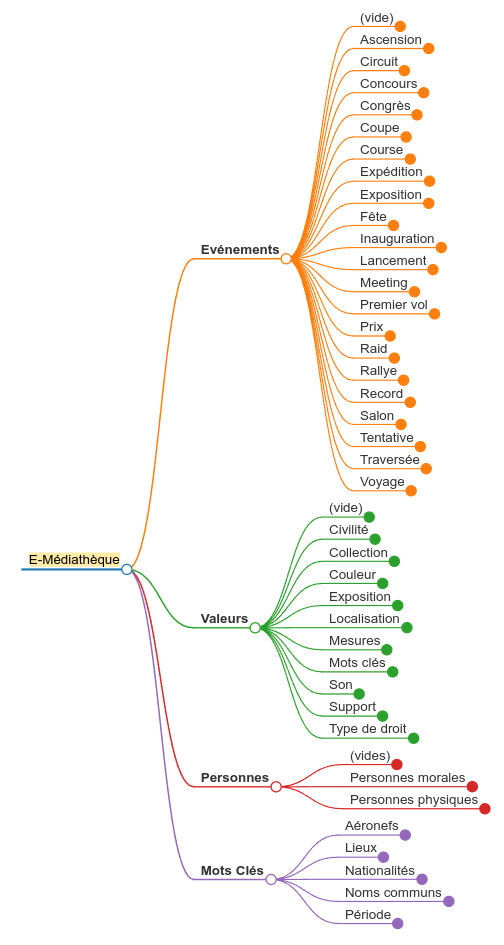
\includegraphics[width=\linewidth]{img/MODEL_emediatheque_arbre}
		\caption{Modélisation en arbre html interactif réalisée avec \textit{markmap}}
		\label{model:arbre-emediatheque}
	\end{subfigure}
	\hfill
	\begin{subfigure}{0.5\textwidth}
		\centering
		\includegraphics[width=\linewidth]{img/GRAPH_emediatheque}
		\caption{Modélisation en graphe réalisée avec \textit{Gephi}}
		\label{model:graph-emediatheque}
	\end{subfigure}
	\caption[Modélisation des \gls{thesaurus} du \mae]{Trois types de modélisations pour un même thésaurus offrent trois approches différentes : notamment, la première permet une vue d'ensemble rapide du type de contenu, la seconde permet d'explorer les branches les unes après les autres, la troisième permet de visualiser des \textit{clusters} de mots -- et pourrait également représenter leurs relations.}
	\label{fig:modelisationthesaurus}
\end{figure}


La visualisation des données par le biais de graphes générés avec Gephi ou d'arbres de concepts interactifs\footnote{Ces arbres, qui auraient également pu être réalisés en Python à l'aide bibliothèques comme \textit{pandas} ou \textit{matplotlib}, ont été réalisés à des fins d'illustration en convertissant un tableau excel en format \textit{markdown} et en générant un fichier html à l'aide de l'application web markmap.} offre une alternative plus intuitive et immédiatement opératoire. Au MAE, ces graphes – qui ont été ensuite mis à disposition de tous les utilisateurs – ont permis de cartographier les clusters thématiques, de détecter les termes orphelins, d'identifier des incohérences dans la hiérarchie des vocabulaires ou des disproportions dans certaines branches du thésaurus. Ils ont servi de support à la restructuration du thésaurus, mais aussi d'outil de médiation entre métiers, lors des groupes de travail ou des ateliers de sensibilisation.

Le format le plus simple -- et donc le plus utilisé, même si moins riche -- a été la modélisation sous forme de \textit{mindmap}, pour représenter seulement les niveaux les plus hauts d'une hiérarchie et travailler sur des grandes catégories de concepts. Celui-ci,  réalisé à partir de logiciels en ligne comme \textit{draw.io}, s'utilise facilement en combinaison avec les tableaux bruts du thésaurus.

On retrouve ici une tension propre à la modélisation documentaire en institution patrimoniale : le compromis entre la formalisation technique – garante de l'interopérabilité et de la pérennité – et la souplesse nécessaire à la prise en main par des agents aux profils variés. Combiner les différents schémas permet ainsi de montrer différents aspects de l'état de l'information au musée, mais aussi de parler à différents profils, et de répondre aux biais, omissions ou transformations inévitables dans toute modélisation et représentation du savoir\footcite{bowkerArrangerChosesConsequences2023}

Ainsi, la modélisation documentaire au \mae – et plus largement dans les institutions patrimoniales – ne saurait se réduire à un exercice technique. Elle est un instrument de dialogue, d'analyse et de gouvernance, dont la réussite dépend de la capacité à articuler exigence conceptuelle et pragmatisme métier, rigueur des normes et souplesse des usages, pour faire du vocabulaire documentaire un espace partagé, vivant et évolutif.

\begin{table}[htbp]
	\caption{Comparatif des visualisations de données utilisées au MAE pendant le stage}
	\label{tab:comparatif_visualisations}
	\centering
	\setlength{\arrayrulewidth}{0.6pt}
	\renewcommand{\arraystretch}{1.3}
	\begin{tabular}{|p{3cm}|p{4cm}|p{4cm}|p{3cm}|}
		\hline
		\rowcolor{lightgray}
		\textbf{Outil / Visualisation} & \textbf{Avantages principaux} & \textbf{Défauts / Limites} & \textbf{Usages / Destinataires} \\
		\hline
		Diagramme UML & Rigueur, structuration, conformité aux normes (ISO 25964), repérage des écarts avec les standards, interopérabilité forte & Complexité du formalisme, peu accessible pour les non spécialistes, jugé "obscur" & Métiers techniques, experts, audit documentaire \\
		\hline
		Graphe Gephi & Intuitif, interactif, cartographie des clusters, identification des orphelins, support à la restructuration, accessible à tous & Moins formel, difficulté à intégrer des métadonnées complexes, préparation nécessaire & Groupes de travail, ateliers, médiation \\
		\hline
		Arbres de concepts (draw.io, markmap, etc.) & Très accessibles, vues d'ensemble, communication institutionnelle, rapide à réaliser & Peu de granularité, perte de précision sur les liens, adapté aux grandes catégories & Sensibilisation, CA, ateliers \\
		\hline
		Tableaux de synthèse (Excel, markdown) & Utilisation universelle, tri et export rapide, support aux corrections, facile à enrichir & Peu visuel, ne cartographie pas les relations, perte du contexte relationnel & Agents, gestionnaires, formation \\
		\hline
	\end{tabular}
\end{table}
 
\subsection{La modélisation comme outil de sensibilisation et de pilotage}

La modélisation conceptuelle n’est pas qu’un acte technique : elle est aussi un instrument de sensibilisation et de pilotage institutionnel. Au \mae, l’organisation d’ateliers a permis d’inviter les agents à réfléchir ensemble à la structuration de l’information, à prendre conscience des enjeux de la donnée et de la transmission documentaire.

Ceux-ci ont utilisé la modélisation pour repenser la hiérarchie des termes ou la nomenclature des vocabulaires. Ce travail a permis de concrétiser aux yeux de tous les métiers l'état des connaissances de l'ensemble du musée, et de réfléchir à la manière de les unifier en un unique système.

Ainsi, la modélisation conceptuelle se révèle être le socle sur lequel peut s’édifier une gouvernance documentaire partagée, une culture commune de l’information, et une capacité à piloter le changement dans la durée.